% Gemini theme
% https://github.com/anishathalye/gemini

\documentclass[20pt, final]{beamer}

% ====================
% Packages
% ====================

%\usepackage[T1]{fontenc}
\usepackage{lmodern}
\usepackage[size=a1, scale=1.0]{beamerposter}
\usetheme{gemini}
\usecolortheme{gemini}
\setbeamerfont{block body}{family=\Lato,size={\fontsize{25}{27}}}
\setbeamerfont{enumerate item}{size={\fontsize{25}{27}}}

\usepackage{graphicx}
\usepackage{booktabs}
\usepackage{tikz}
\usepackage{pgfplots}
\usepackage{fontawesome}
\pgfplotsset{compat=1.14}
\usepackage{anyfontsize}

\usepackage{tcolorbox}

\usepackage{wrapfig}
\usepackage{braket}
\usepackage{bm}


%% ---------- useful for the schema ---------

\usetikzlibrary{positioning,arrows,calc,math,angles,quotes}
\usetikzlibrary{arrows,automata}
\usetikzlibrary{positioning}
\usetikzlibrary{arrows.meta,
                bending,
                intersections,
                quotes,
                shapes.geometric}

\tikzset{
    state/.style={
           rectangle,
           rounded corners,
           draw=black, very thick,
           minimum height=1em,
           inner sep=2pt,
           text centered,
           },
}



\definecolor{darkmidnightblue}{rgb}{0.0, 0.2, 0.4}

% ====================
% Lengths
% ====================

% If you have N columns, choose \sepwidth and \colwidth such that
% (N+1)*\sepwidth + N*\colwidth = \paperwidth
\newlength{\sepwidth}
\newlength{\colwidth}
\setlength{\sepwidth}{0.025\paperwidth}
\setlength{\colwidth}{0.3\paperwidth}


% useful for the logos

\logoright{
\includegraphics[height=4cm]{figures/qr-code.png}}
\logoleft{
\includegraphics[height=4cm]{figures/qibo_qr.png}}


\newcommand{\separatorcolumn}{\begin{column}{\sepwidth}\end{column}}

% ====================
% Title
% ====================

\title{Determining probability density functions with adiabatic quantum computing}

\author{Robbiati M. \inst{1  }\inst{2  }, Cruz-Martinez J. M. \inst{2  }, \and Carrazza S. \inst{1  }\inst{2  }\inst{3    }}

\institute[shortinst]{
  \inst{1  } TIF Lab, Dipartimento di Fisica, Universit\`a degli Studi
  di Milano, Milan, Italy. 
  \samelineand 
  \inst{2  } CERN, Theoretical Physics Department, CH-1211
  Geneva 23, Switzerland.
  \samelineand
  \inst{3  } Quantum Research Center, Technology Innovation Institute, Abu Dhabi, UAE.
  }

% ====================
% Footer (optional)
% ====================

\footercontent{
}
% (can be left out to remove footer)

% ====================
% Logo (optional)
% ====================

% use this to include logos on the left and/or right side of the header:
% \logoright{\includegraphics[height=7cm]{logo1.pdf}}
% \logoleft{\includegraphics[height=7cm]{logo2.pdf}}

% ====================
% Body
% ====================

\begin{document}

\begin{frame}[t]
\begin{columns}[t]
\separatorcolumn

\begin{column}{\colwidth}

  \begin{block}{Abstract}

   We present a method for estimating Probability Density Functions (PDFs) of one dimensional
   samples using adiabatic quantum computing. We use an adiabatic evolution
   to encode the cumulative distribution (CDF), exploiting the natural monotonicity of
   the evolution and choosing the boundary Hamiltonians to perfectly fit the target
   problem. We then translate the evolution into a continuous-in-time circuit 
   using a Trotter-like procedure. Finally, we derivate the circuit using the Parameter
   Shift Rule (PSR) in order to get the PDF.
  \end{block}

  \begin{alertblock}{Goal}

    Estimating the PDF value $\rho(x)$ for each element of a sample of data
    $\Omega=\{x_j\}_{j=1}^{N_{\rm data}}$.  We define the following Quantum 
    Adiabatic Machine Learning (QAML) strategy:
    
    \begin{itemize}
    \item[\faChain] encoding the CDF values $F(x)$ into an adiabatic evolution;
    \item[\faPencil] translating the adiabatic Hamiltonian into a circuit 
    $\mathcal{C}$ callable at any time $\tau$;
    \item[\faCogs] Derivating the circuit using the parameter shift 
    rule~\cite{Schuld_2019} obtaining the PDF. 
    \end{itemize}

  \end{alertblock}


  \begin{block}{\faChain\,\, Encoding a CDF into an adiabatic evolution}

  We use \texttt{qibo}~\cite{Efthymiou_2021} to simulate an adiabatic evolution on time $\tau$:
  \begin{equation}
  H_{\rm ad}(\tau, \bm{\theta}) = \bigl[ 1 - s(\tau, \bm{\theta}) \bigr] H_0 + 
  s(\tau, \bm{\theta}) H_1. 
  \end{equation}

  We map $\{x, F(x)\}$ into $\{\tau, E(\tau)\}$ , where $E(\tau)$ energy of a 
  non-interacting Pauli Z over the evolved ground state of $H_{\rm ad}$ at $\tau$.

  \begin{figure}
    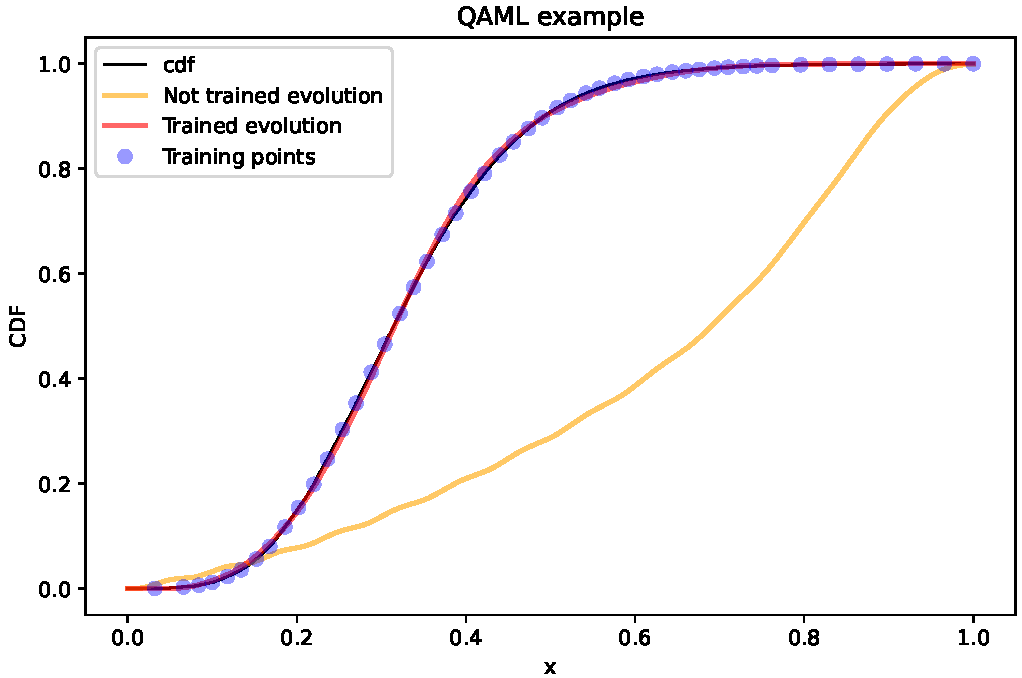
\includegraphics[width=0.7\textwidth]{figures/evolution.pdf}
  \end{figure}
  \end{block}

  \begin{alertblock}{How we optimize the evolution}
  
  \begin{enumerate}
    \item perform the evolution with initial guess $\bm{\theta}_0$ in the scheduling;
    \item estimating a loss function $J_{\rm mse}\bigl[F, E(\bm{\theta})\bigr]$;
    %\begin{equation*} 
    %J_{\rm mse} \frac{1}{N_{data}} \sum_{k=1}^{N_{data}} \bigl[ E(\tau_k) - 
    %F(x_k)\bigr];
    %\end{equation*} 
    \item updating $\bm{\theta}$ using a chosen optimizer until convergence.
  \end{enumerate}

  \end{alertblock}


\end{column}

\separatorcolumn

\begin{column}{\colwidth}

  \begin{block}{\faPencil, \faCogs\,\, Building a derivable circuit}
  
After encoding the CDF into the evolution, we translate $H_{\rm ad}$ into a circuit
derivable via PSR:

\begin{tikzpicture}[->,>=stealth']

\vspace{5cm}


    \node[
      state, 
      xshift=-1cm] (CDF) 
        {
          \begin{tabular}{l}
        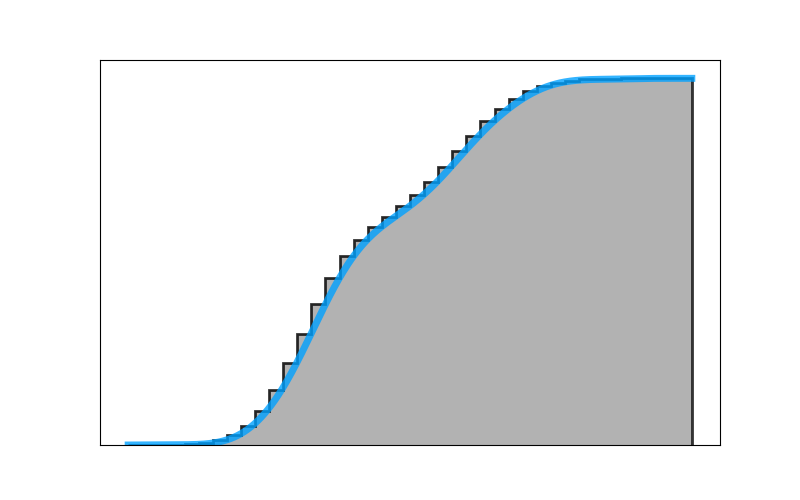
\includegraphics[width=0.3\textwidth]{figures/cdf.png}
          \end{tabular}
    };
 % base node: the adiabatic evolution 
  \node[
    state, 
    right of=CDF, 
    xshift=-2cm,
    yshift=0cm, 
    anchor=center, 
    node distance=13.8cm, 
    fill=blue!15,
    label={Sequence of $\{H_j\}$}] (AE)
    {
      \begin{tabular}{l}
        \parbox{10.5cm}{$$\hat{F}(x) \to \ket{\psi(\tau)} = \prod_{j}^{\leftarrow} U_j \ket{\psi_0}$$}\\
      \end{tabular}
    };

% continuous limit: jumping to a circuit
  \node[
    state, 
    below of=AE, 
    yshift=0cm,
    xshift=2cm, 
    anchor=center, 
    node distance=7cm, 
    fill=blue!15, 
    label={$d\tau \to 0$ limit}] (U) 
      {
        \begin{tabular}{l}
          \parbox{8cm}{$$ \ket{\psi(\tau)} = \mathcal{C}(\tau) \ket{\psi_0} $$}\\
        \end{tabular}
      };

      % rotational gates
  \node[
    state, 
    left of=U, 
    xshift=-7cm, 
    anchor=center, 
    node distance=6cm, 
    fill=blue!15, 
    label={From $\mathcal{C}$ to $\mathcal{C}_R$}] (Rot) 
    {
      \begin{tabular}{l}
        \parbox{12cm}{$$\ket{\psi(\tau)} = R_z(\theta_1) R_x(\theta_2) R_z(\theta_3) \ket{\psi_0} $$}\\
        with $\theta_i\equiv \theta \bigl(s(\tau)\bigr)$.
      \end{tabular}
    };

    \node[
    state, 
    below of=Rot, 
    xshift=0cm,
    yshift=0cm, 
    anchor=center, 
    node distance=7cm, 
    fill=blue!15, 
    label={Derivative of $\mathcal{C}_R$}] (PSR) 
    {
      \begin{tabular}{l}
        \parbox{10cm}{$$ \rho(x) = \partial_{\tau} \hat{F} = \sum_{i=1}^3 \frac{\partial 
        \hat{F}}{\partial \theta_i}\frac{\partial \theta_i}{\partial \tau}
          $$}\\
        where $\frac{\partial \hat{F}}{\partial \theta_i}$ with PSR
      \end{tabular}
    };

    \node[
    state, 
    right of=PSR, 
    xshift=0cm,
    yshift=0cm, 
    anchor=center, 
    node distance=12cm] (PDF) 
        {
          \begin{tabular}{l}
        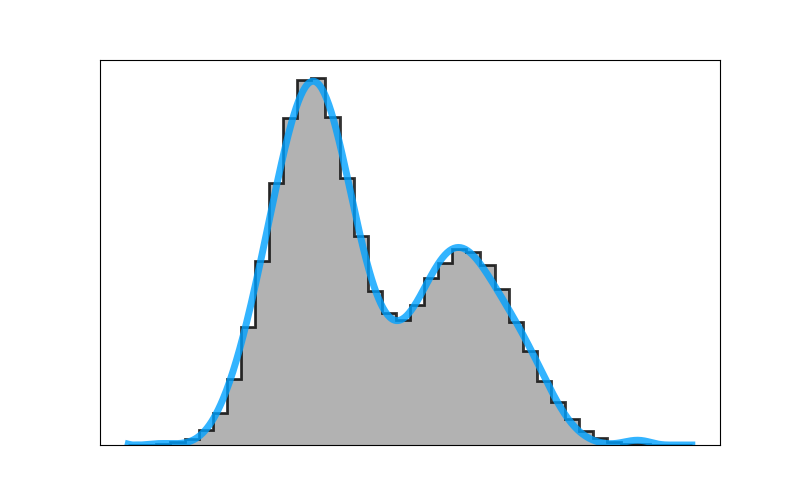
\includegraphics[width=0.3\textwidth]{figures/pdf.png}
          \end{tabular}
    };

\draw[line width=0.8mm] (3.5, 0)  to[out=0, in=180] (5.0, 0);
\draw[line width=0.8mm] (16.6, 0)  to[out=340, in=45] (17.1, -5.5);
\draw[line width=0.8mm] (8, -7)  to[out=180, in=0] (6.4, -7);
\draw[line width=0.8mm] (-6.8, -9)  to[out=250, in=140] (-6.2, -13.2);
\draw[line width=0.8mm] (5.4, -14)  to[out=0, in=180] (7.2, -14);
\end{tikzpicture}

\end{block}




  \begin{block}{Validation cases}

  We firstly test the QAML procedure on a Gamma distribution and on a Gaussian 
  mixture.

    \begin{figure}
    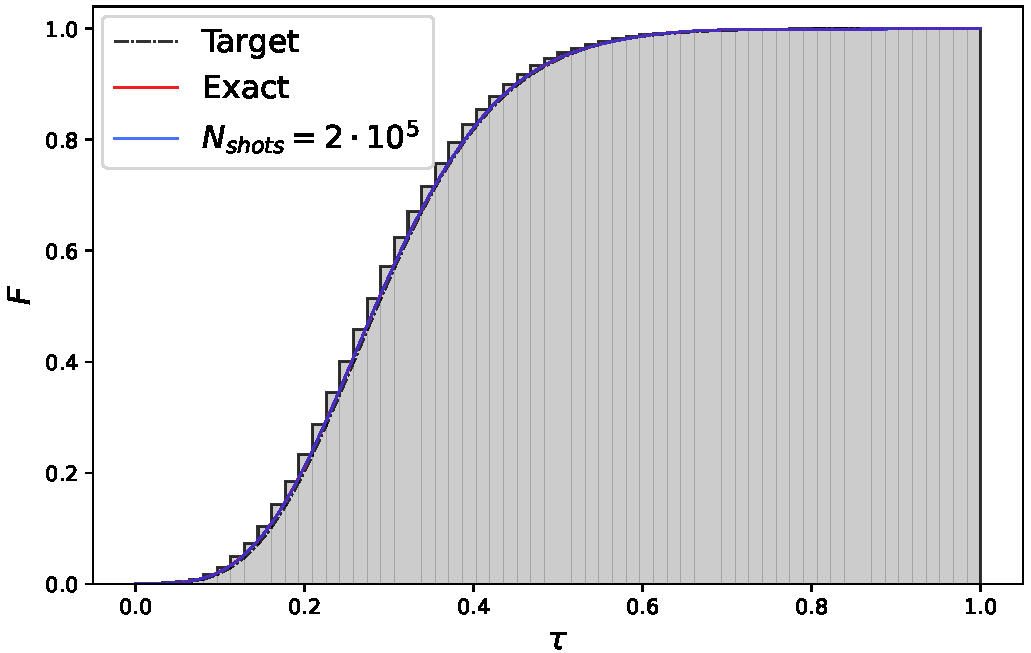
\includegraphics[width=0.5\textwidth]{figures/gamma_cdf.pdf}%
    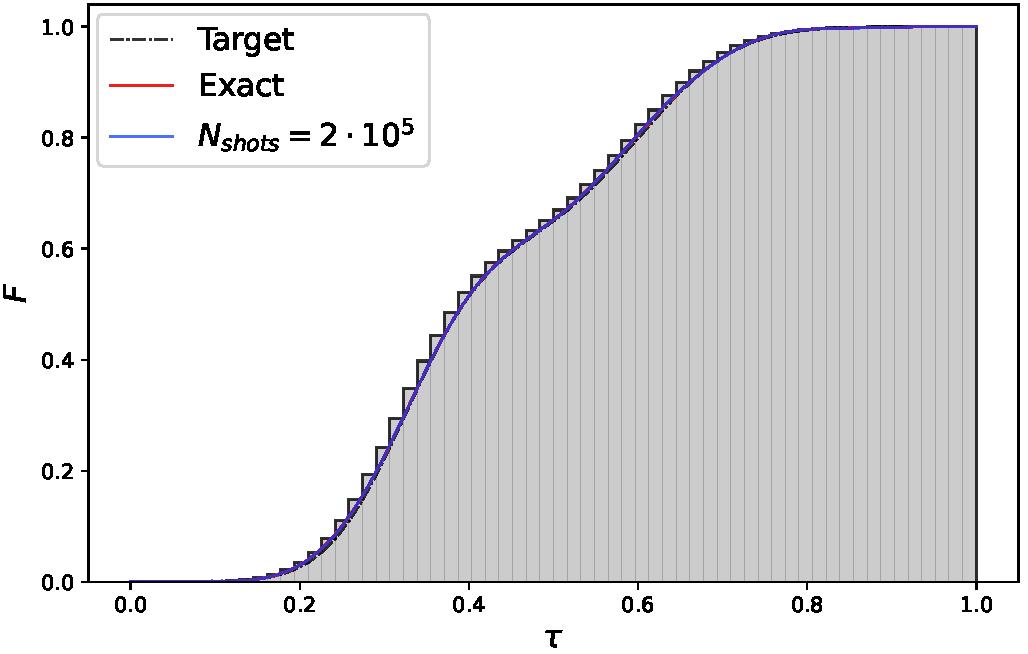
\includegraphics[width=0.5\textwidth]{figures/gauss_cdf.pdf}
    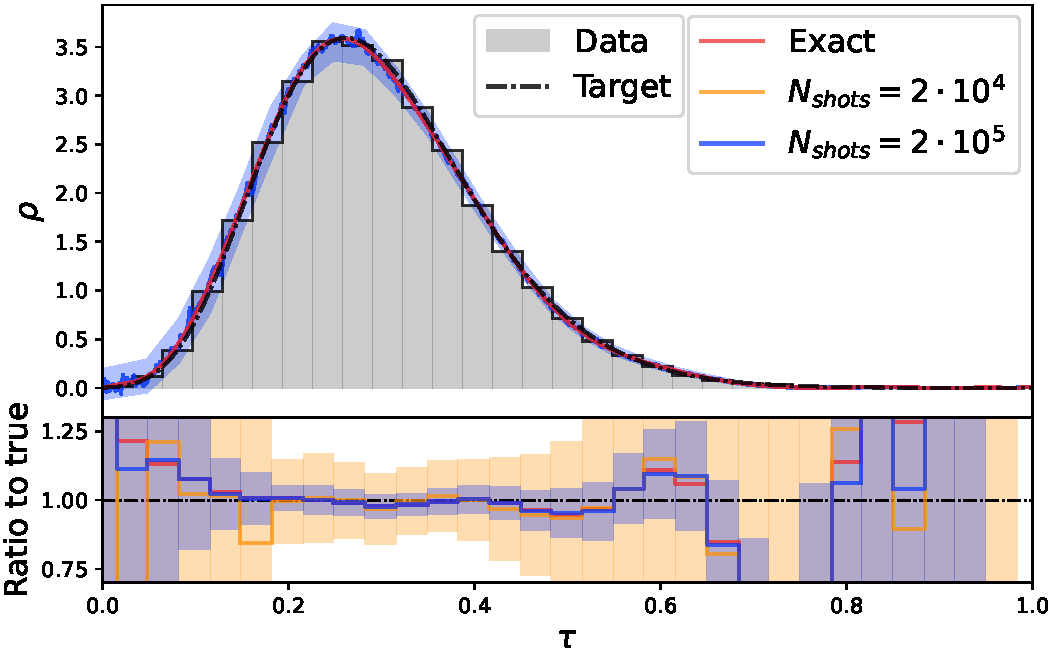
\includegraphics[width=0.5\textwidth]{figures/gamma_pdf.pdf}%
    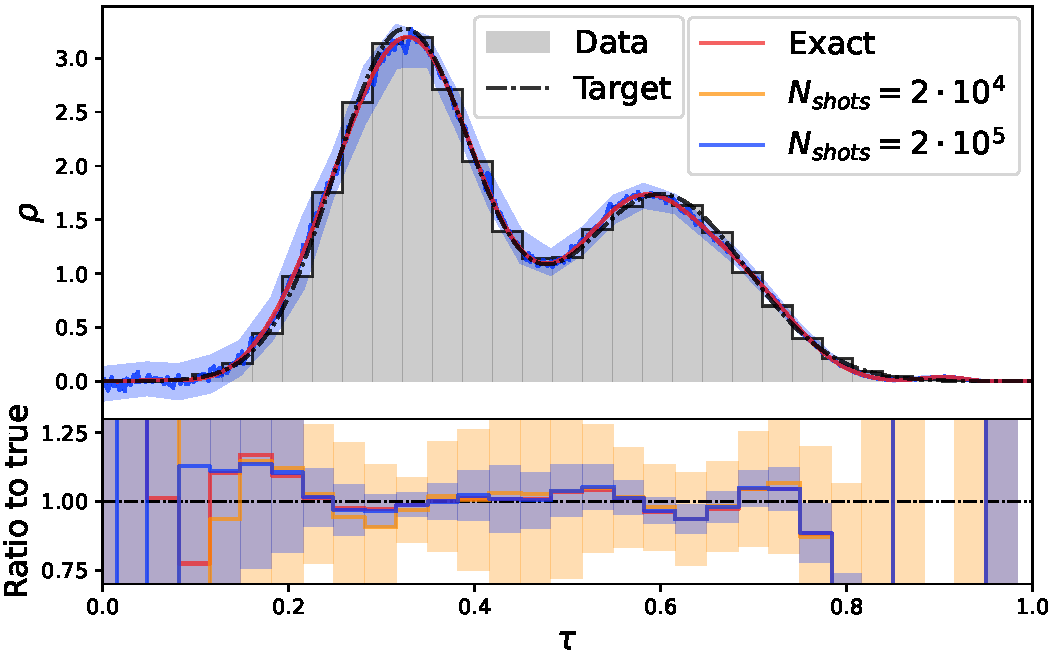
\includegraphics[width=0.5\textwidth]{figures/gauss_pdf.pdf}
    \end{figure}

  \end{block}

\end{column}

\separatorcolumn

\begin{column}{\colwidth}

  \begin{block}{Quantum density estimation after quantum data generation}

  LHC events of a $pp\to t\bar{t}$ decay generated with a quantum 
  GAN~\cite{Bravo_Prieto_2022}. 

    \begin{figure}
    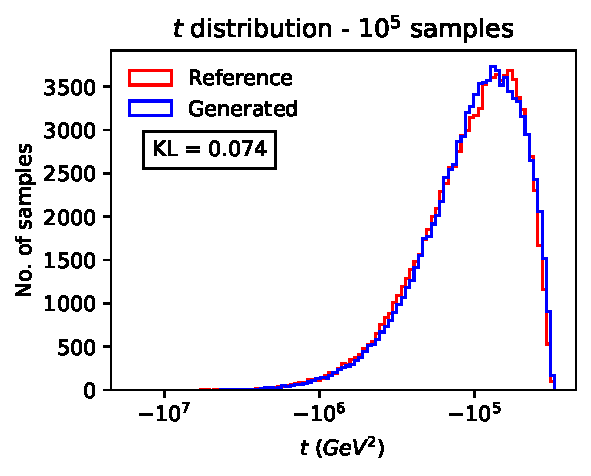
\includegraphics[width=0.5\textwidth]{figures/t_qgan.pdf}%
    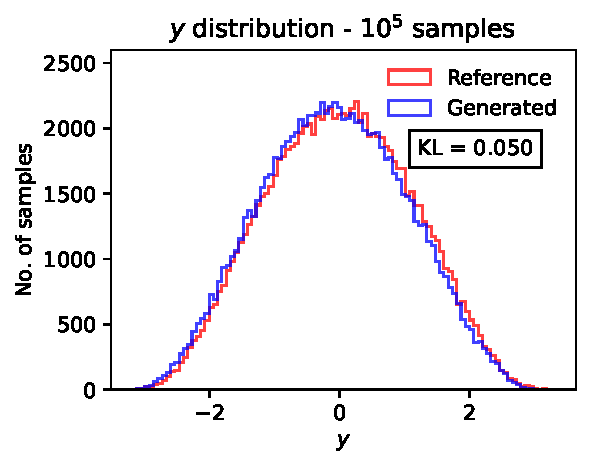
\includegraphics[width=0.5\textwidth]{figures/y_qgan.pdf}%
    \end{figure}

  On which we apply the QAML algorithm:

    \begin{figure}
    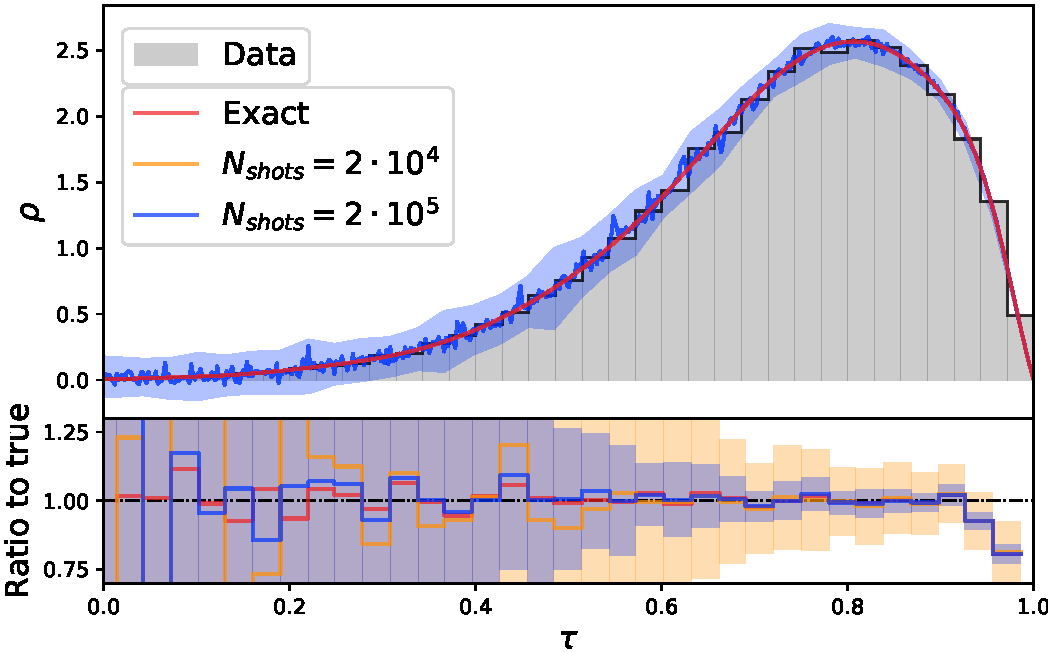
\includegraphics[width=0.5\textwidth]{figures/t.pdf}%
    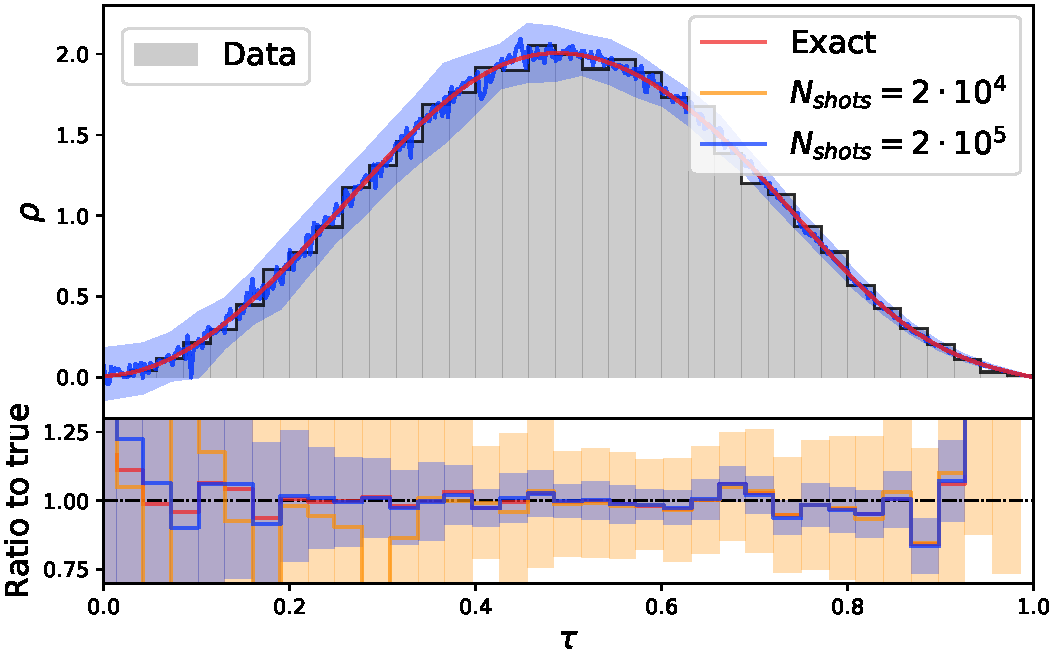
\includegraphics[width=0.5\textwidth]{figures/rapidity.pdf}%
    \end{figure}
    

  \end{block}

  \begin{alertblock}{Results}
Simulation with shots noise due to $N_{\rm nshots}=5\cdot 10^4$.
\vspace{1cm}
  \begin{center}
  \begin{tabular}{lccccc}
  \hline \hline
    Fit function & $N_{\rm sample}$ & $p$ & $J_f$ & $N_{\rm ratio}$ & $\chi^2$\\
  \hline
    Gamma & $5 \cdot 10^4$ & $25$ & $2.9 \cdot 10^{-6}$ & $31$ & $2.2\cdot10^{-4}$ \\
    Gaussian mix & $2 \cdot 10^5$ & $30$ & $2.75 \cdot 10^{-5}$ & $31$ & $4.39 \cdot 10^{-3}$ \\
    $t$ & $5\cdot 10^4$ & $20$ & $2.1 \cdot 10^{-6}$ & $34$ & $3.4 \cdot 10^{-4}$ \\
    $s$ & $5\cdot 10^4$ & $20$ & $7.9 \cdot 10^{-6}$ & $34$ & $1.20 \cdot 10^{-3}$\\
    $y$ & $5\cdot 10^4$ & $8$ & $3.7 \cdot 10^{-6}$ & $34$ & $1.45 \cdot 10^{-3}$\\
  \hline \hline
  \end{tabular}
\end{center}

  \end{alertblock}

  \begin{block}{References}
  \nocite{*}
    \small  {\bibliographystyle{plain}\bibliography{poster.bib}}
  \end{block}

\end{column}

\separatorcolumn
\end{columns}
\end{frame}

\end{document}
